\documentclass[12pt,italian]{article}
\usepackage{babel}
\usepackage[T1]{fontenc}
\usepackage[utf8]{inputenc}
\usepackage{amsmath}
\usepackage{graphicx}

\title{
    Controlli Automatici T \\
    \large Progetto gruppo AO --- traccia 3c\\
}
\author{
    Giacomo Romanini\\
    \and
    Guglielmo Palaferri\\
    \and
    Luca Tacinelli\\
    \and
    Pietro Girotti\\
}
\date{30 giugno 2021}

\begin{document}
\maketitle

\begin{figure}[h]
    \begin{center}
        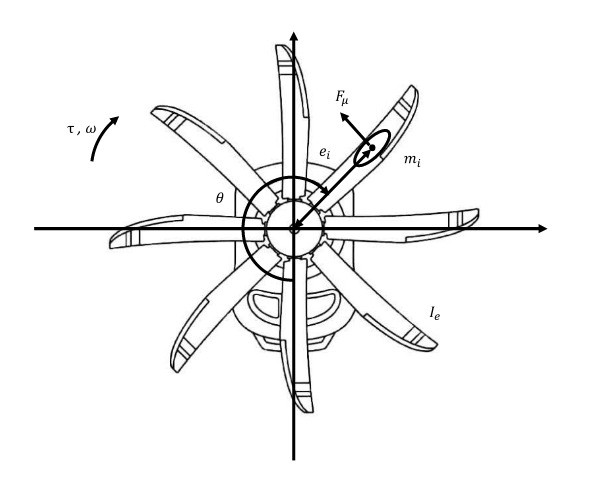
\includegraphics[scale=0.5]{elica.png}
        %\caption{Rappresentazione grafica del sistema (elica)}
    \end{center}    
\end{figure}

\newpage

\section{Linearizzazione nell'intorno di $(x_e, u_e)$}
Il sistema del motore ad elica assegnato è descritto dalle seguenti equazioni: 

\begin{equation}
    \begin{aligned}
        \dot{\theta} &= \omega\\
        (m_i e_i^2 + I_e)\dot{\omega} &= -\beta \omega - \mu_d m_i \omega^2 e_i^2 + \tau
    \end{aligned}
\end{equation}
dove si considerano
\begin{align*}
    &x(t) =
    \begin{bmatrix}
        x_1(t)\\
        x_2(t)
    \end{bmatrix} =
    \begin{bmatrix}
        \theta(t)\\
        \omega(t)
    \end{bmatrix}\\
    &u(t) = \tau(t)\\
    &y(t) = \omega(t)
\end{align*}
\\
Sostituendo i parametri è possibile ottenere le equazioni di stato:
\begin{equation}
    \begin{aligned}
        \dot{x_1}(t) &= x_2(t)\\
        \dot{x_2}(t) &= -\frac{\beta}{(m_i e_i^2 + I_e)} x_2(t) - \frac{\mu_d m_i e_i^2}{(m_i e_i^2 + I_e)} x_2^2(t) + \frac{1}{(m_i e_i^2 + I_e)}u(t)
    \end{aligned}
\end{equation}
\\
Inoltre, poiché la dinamica di $\theta$ è ininfluente per l'evoluzione del sistema, si conosce $x_e = 
\begin{pmatrix}
    0\\
    10000/2\pi
\end{pmatrix}$
e $y_e = \omega_e = 10000/2\pi$







\end{document}